\documentclass{beamer}

\usepackage{agda}
\usepackage{apacite}
\usepackage{catchfilebetweentags}
\usepackage{changepage}
\usepackage{babel}

\usepackage{graphicx}

\usepackage[autostyle=true,french=guillemets,maxlevel=3]{csquotes}

\graphicspath{ {images/} }
 
\usetheme{Frankfurt}

\DeclareQuoteStyle{english}
  {\em}
	{\em}
	{\textquotedblleft\em}
	{\em\textquotedblright}

 
%Information to be included in the title page:
\title{Qualificação}
\author[Guilherme, Flávio]{Guilherme Horta Alvares da Silva \\
  Orientador: Flávio Codeço Coelho}
\institute{Fundação Getulio Vargas}
\date{2019}

 
\begin{document}
 
\frame{\titlepage}

\begin{frame}
  \frametitle{Programação de uma criptomoeda em linguagem Agda}
\begin{itemize}
  \item Objetivo
  \item Justificativa
  \item Introdução
  \begin{itemize}
    \item Criptomoedas
    \item Agda
    \item Bugs em criptomoedas
  \end{itemize}
  \item Trabalho executado
  \item Próximos passos
  \item Referências Bibliográficas
\end{itemize}
\end{frame}

\section{Objetivo}

 \begin{frame}
\frametitle{Objetivo}
\begin{itemize}
  \item Programar uma criptomoeda (similar ao Bitcoin) em Agda, que é uma linguagem com tipos dependentes.
    %% 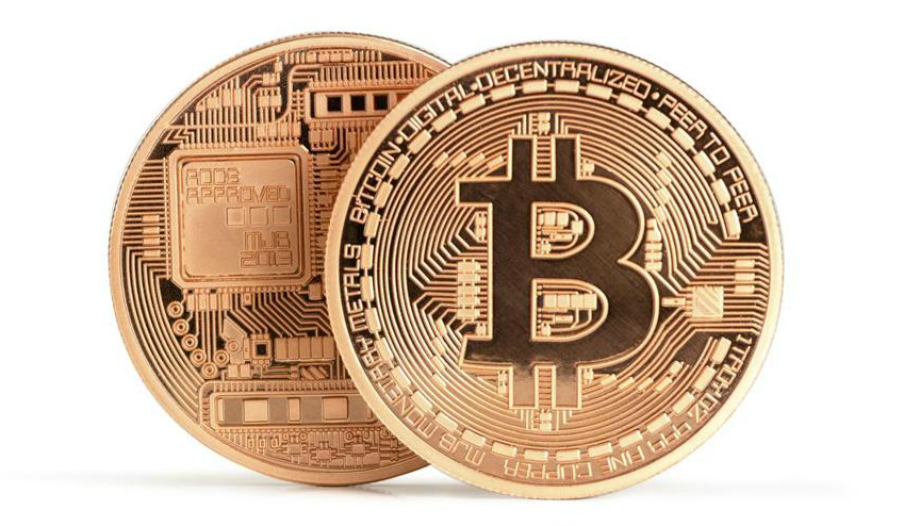
\includegraphics[width=8cm, height=5cm]{TwoBitcoins}
\end{itemize}
\end{frame}
 
\section{Justificativa}

 \begin{frame}
\frametitle{Justificativa}
\begin{itemize}
    \item Programar um protocólo de criptomoedas livre de erros (bugs)
    \item Utilizar Agda permite, além da programação da criptomoeda, especificar como ela deve funcionar
      \cite{norell2008dependently}
\end{itemize}
\end{frame}

\section{Criptomoedas}

\begin{frame}
  \frametitle{Criptomoeda}
\begin{itemize}
    \item Uma criptomoeda é um meio de troca descentralizado que se utiliza da tecnologia de blockchain e da criptografia para assegurar a validade das transações e a criação de novas unidades da moeda
    \item O bitcoin é considerado a primeira moeda digital mundial descentralizada, constituindo um sistema econômico alternativo (\foreignquote{english}{peer-to-peer electronic cash system}) e responsável pelo ressurgimento do sistema bancário livre
      \cite{nakamoto2008bitcoin}
    \item O Bitcoin permite transações financeiras sem intermediários, mas verificadas por todos usuários (nodos da rede). Estas transações são gravadas em um banco de dados distribuídos (uma rede descentralizada), chamado de \foreignquote{english}{blockchain}.
    \end{itemize}
\end{frame}

\begin{frame}
\frametitle{Blockchain}
%% 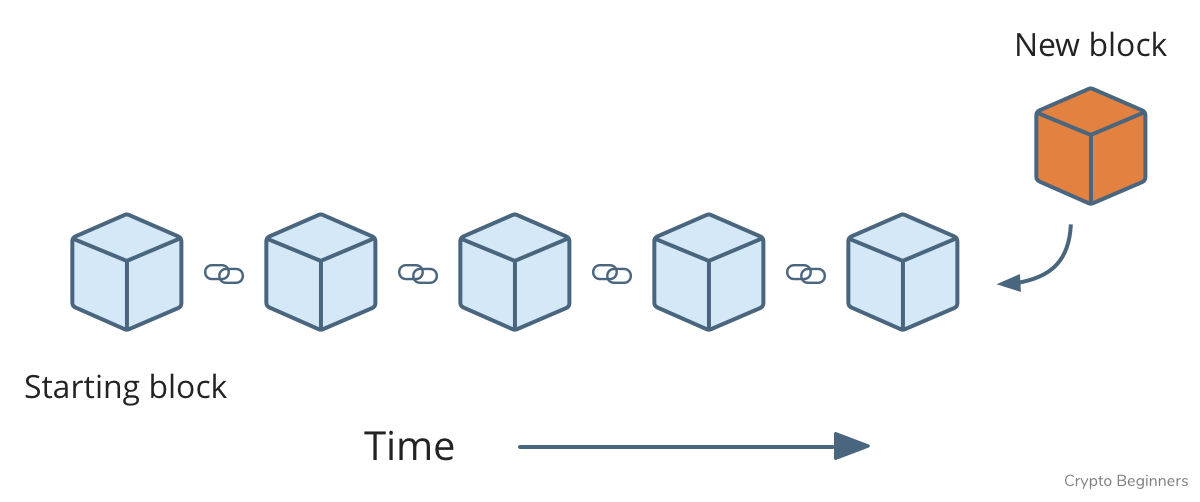
\includegraphics[width=11cm, height=8cm]{blockchain1}
\end{frame}

\begin{frame}
\frametitle{Blockchain}
%% 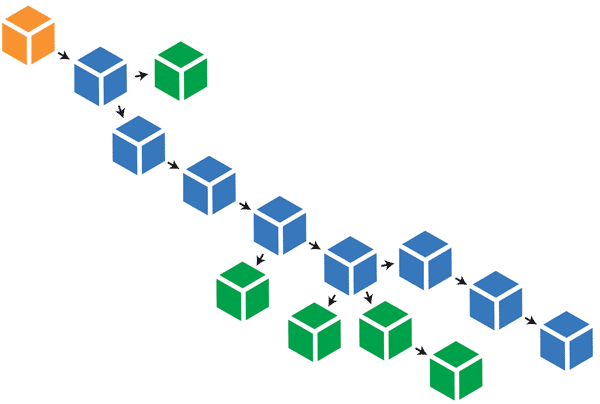
\includegraphics[width=11cm, height=8cm]{blockchain2}
\end{frame}

\begin{frame}
\frametitle{Blockchain}
%% 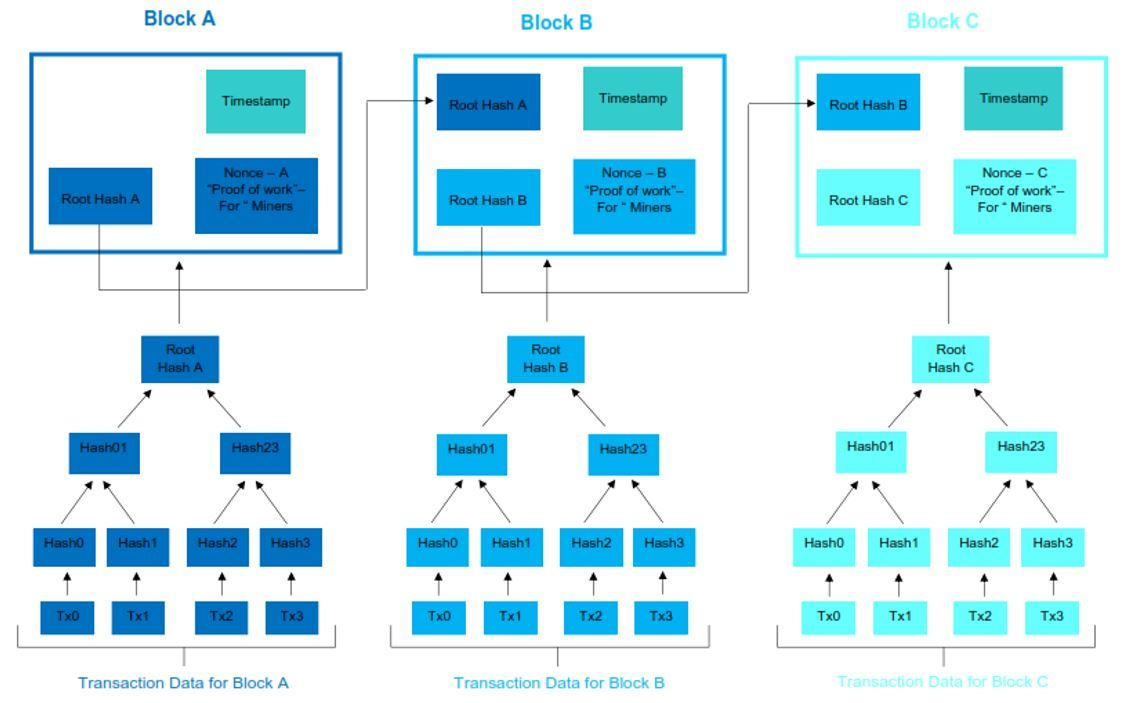
\includegraphics[width=11cm, height=8cm]{blockchain3}
\end{frame}
 
\section{Agda}

 \begin{frame}{Agda}
 \begin{itemize}
   \item Linguagem funcional com sistema de tipos expressivos capazes de representar as especificações
     \item Possibilita especificar e programar em um único lugar
     \item O processo de verificação acontece no compilador
 \end{itemize}
 \end{frame}
 
 \begin{frame}{Agda --- II}
 \begin{itemize}
     \item A linguagem não possui \foreignquote{english}{Built-in} como em Python
     \item Tipos como inteiros, ponto flutuantes, \foreignquote{english}{strings} e vetores devem ser definidos pelo próprio usuário
     \item Tipos em Agda são uma generalização de tipos de dados algébricos encontrados em Haskell e ML
 \end{itemize}
 \end{frame}
 
 \begin{frame}{Agda --- III}
\begin{itemize}
  \item Definição dos números naturais como axiomas de Peano:
           %% \ExecuteMetaData[latex/Code.tex]{nat}
 \end{itemize}
\end{frame}

\begin{frame}{Agda --- IV}
 \begin{itemize}
   \item Adição em Agda:
 \end{itemize}
 %% \ExecuteMetaData[latex/Code.tex]{plus}
\end{frame}

\begin{frame}{Agda --- V}
 \begin{itemize}
   \item Um tipo é dependente se este depende de um valor.
   \item Exemplo --- Listas indexadas por seu tamanho:
 \end{itemize}
 %% \ExecuteMetaData[latex/Code.tex]{vector}
\end{frame}

\begin{frame}{Agda --- VI}
 \begin{itemize}
   \item Modo seguro de remover primeiro elemento do vetor:
     %% \ExecuteMetaData[latex/Code.tex]{vectorhead}
   \item Função zip com 2 vetores de mesmo tamanho:
     %% \ExecuteMetaData[latex/Code.tex]{zipWith}
 \end{itemize}
\end{frame}

\section{Bug}

 \begin{frame}
   \frametitle{Maleabilidade de transacao}
\begin{itemize}
  \item Nesse tipo de bug, é possível alterar o hash da transação depois que ela foi enviada
  \item Todos os dados para calcular do hash não eram previamente calculados. Assim, o minerador poderia alterar o hash da transação
  \item O ataque consistiria de um usuário enviar uma transação e ela não ser confirmada pelo sistema.
    Logo em seguida, este mesmo usuário enviaria uma outra transação. Desta forma, ele faria duas transações com a mesma moeda
  \item Este tipo de BUG pode ser evitado usando tipos dependentes. Colocando como característica da transação, o fato de seu ID ser único
\end{itemize}
\end{frame}

\begin{frame}
  \frametitle{DAO Bug}
  \begin{itemize}
    \item \foreignquote{english}{Bug} que aconteceu em um cripto-contrato da rede Ethereum com um prejuízo de mais do que 250 milhões de dólares
      \cite{wood2014ethereum}
    \item No cripto-contrato, existia uma função recursiva que não terminava. Ou seja, o usuário enviava uma quantidade de ethereum, depois acontecia um \foreignquote{english}{loop} infinito e só depois era feito a atualização do seu balanço
    \item Em Agda, esse tipo de bug seria evitado, pois é necessário provar que a função termina. Logo, \foreignquote{english}{loops} infinitos não são possíveis em Agda
  \end{itemize}
\end{frame}

\section{Trabalho executado}

\begin{frame}{Trabalho já executado}
  \begin{itemize}
    \item A criptomoeda já foi programada em Python
    \item Parte da \foreignquote{english}{blockchain} já foi programada em Agda
    \item As transações já foram descritas na literatura: UTXO (\foreignquote{english}{Unspent transaction output}) \\
      \cite{setzer2018modelling}
  \end{itemize}
\end{frame}

\begin{frame}{Blockchain em Agda}
  \begin{adjustwidth}{-3.5em}{-2em} \fontsize{8}{11}
     %% \ExecuteMetaData[latex/Code.tex]{blockchain}
  \end{adjustwidth}
\end{frame}
  
\section{Próximos Passos}

\begin{frame}{Próximos passos}
  \begin{itemize}
    \item Anexar a \foreignquote{english}{blockchain} às transações já programadas em Agda
    \item Provar alguns teoremas relacionados à criptomoeda
  \end{itemize}
\end{frame}

\begin{frame}{Teoremas}
  \begin{itemize}
    \item Se uma transação tem algum \foreignquote{english}{output} que não foi usado em nenhuma outra transação, 
      então ela deve estar na lista de \foreignquote{english}{outputs transactions} não usados
    \item Se uma transação tem algum \foreignquote{english}{output} que foi gasto, ele não pode ser usado novamente
      \item Provar que transações e mensagens ids são únicos
  \end{itemize}
\end{frame}

\begin{frame}{O que não será realizado}
  \begin{itemize}
    \item Modelo de criptomoeda em que é possível algum tipo de \foreignquote{english}{fork}. Por exemplo, no bitcoin, é possível que exista algum tipo de \foreignquote{english}{fork} temporário
    \item \foreignquote{english}{Pool} de transações. Sua utilidade é apenas para guardar as transações que ainda não foram adicionadas a \foreignquote{english}{blockchain}
    Isso pode ser feito fora do protocolo principal
  \item Otimização e protocolos RPC (\foreignquote{english}{Remote Procedure Call}). O objetivo do projeto é definir as propriedades da criptomoeda, não como ela será implementada e usada
  \end{itemize}
\end{frame}

\section{Bibliografia}

 \begin{frame}{Livros}
    %% 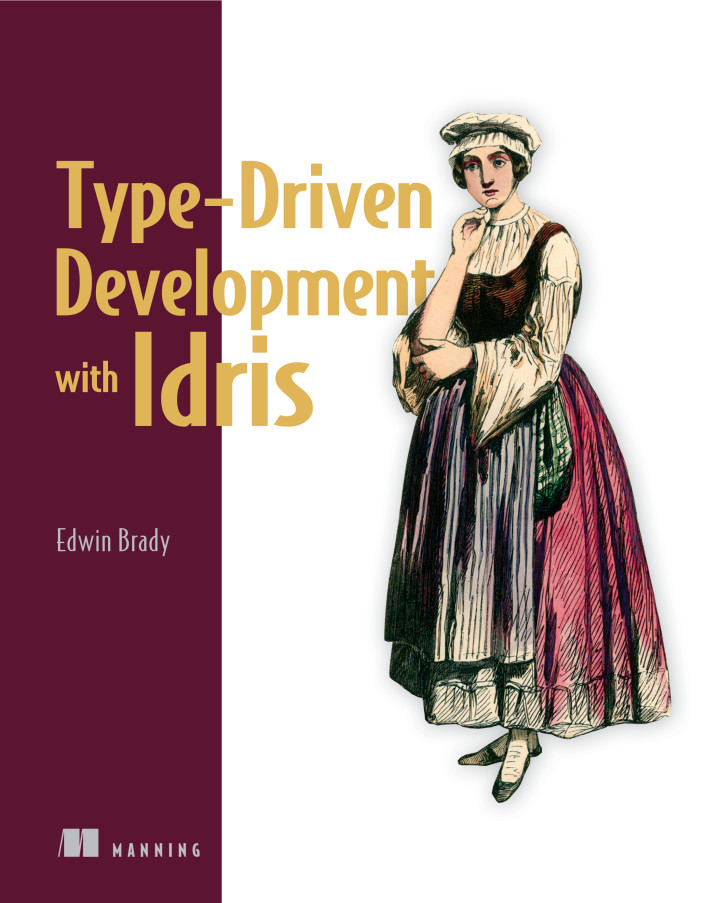
\includegraphics[width=4cm, height=6cm]{TDD}
    %% 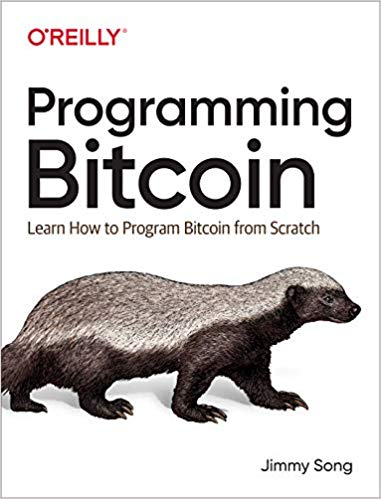
\includegraphics[width=4cm, height=6cm]{ProgrammingBitcoin}
 \end{frame}
  

\begin{frame}{Referências Bibliográficas}
  \bibliographystyle{apacite}
  \bibliography{References}
\end{frame}

\end{document}
